\section{Data association}
\subsection{Choice of method}

\subsection{Design}
The chosen design for the frontend uses ideas from the PDA and compatibility test methods, while simplifying a bit because of the inherent limitiations of the specific problem being solved. The main idea is to compare with the latest map coming out of SLAM, using a compatibility test to associate new measurements with existing landmarks. The measurements that can't be associated to the map are then compared with a list of hypotheses, using the same compatibility test. A hypothesis that gets a new measurement associated to it gets its confidence increased, while the ones that don't get their confidence decreased. The measurements that couldn't get associated to neither the map nor the list of hypotheses gets added to the list of hypotheses. 

Each measurement coming out of the detection algorithms has a covariance matrix that, in the detection frame (see figure \ref{Fig:DetectionFrame}), is empirically found to be approximately a diagonal matrix where the two diagonal elements are functions of distance. 

\todo{Fix these placeholder plots and change the text a bit.}

The dependence of the variance on distance is found by placing cones in a known grid and having their position measured as accurately as possibly. Data from the sensors are then recorded and the detection algorithms give their best estimate of the position of the cones. The many measured cones are then binned together with regards to distance, and the errors in bearing and angle is plotted, as can be seen in figures \ref{Fig:CameraRError} and \ref{Fig:CameraPsiError}. The variance of these predictions are then plotted, shown in figures \ref{Fig:CameraRVariance} and \ref{Fig:CameraPsiVariance}. 

The plots clearly show that the variance in distance and angle is a function of distance, which also logically makes sense. A curve is therefore fitted on top of this. A linear fit was found to be best for the variance of the pure geometrically calculated distance estimate, while a second order polynomial was found to give the best fit for the neural net solution. These fits are plotted in figure \ref{Fig:CameraRVarianceFit}. For the variance in the angle however, both the purely geometrically calculated value and the neural net solution got a second order polynomial. These fits are shown in \ref{Fig:CameraPsiVarianceFit}.

Similar analysis are done for the two other detection algorithms. This means that when a set of new measurements arrive at the SLAM frontend they consist of a vector of measurements and their covariance matrix in the detection frame. 

The covariance matrices in the detection frame, $\Sigma_{detect}$, are then rotated into the body frame using the following formula

\begin{equation}
    \Sigma_{body} = R^T(\alpha)\Sigma_{detect}R(\alpha)
    \label{DetectToBodyRot}
\end{equation}

where 

\begin{equation}
    R(\alpha) = \begin{bmatrix} cos(\alpha) & -sin(\alpha) \\ sin(\alpha) & cos(\alpha)
    \end{bmatrix}
\end{equation} 

and $\alpha$ is the angle between the x-axis of the body frame and the line between CG and the cone in question. 

\begin{figure}
    \centering
    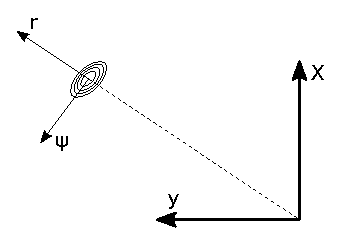
\includegraphics[width=0.5\linewidth]{0_Images/3_Theory/DetectionFrame.eps}
    \caption[The detection frame.]{The detection frame, body frame and height curves of the gaussian noise on the detected cones position.}
    \label{Fig:DetectionFrame}
\end{figure}

\iffalse
\begin{figure}
    \centering
    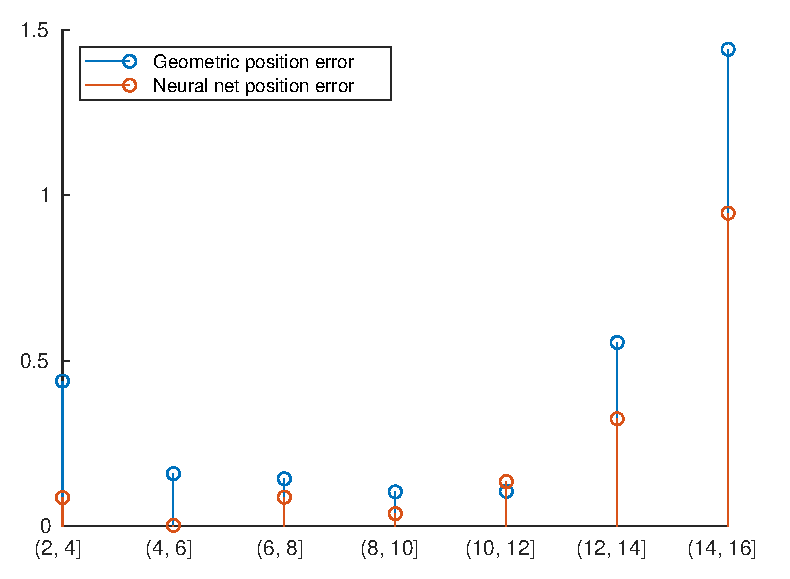
\includegraphics[width=0.5\linewidth]{0_Images/3_Theory/camDetection/rErrorCamera.eps}
    %\captionof{figure}{The error and variance along the r-direction of the camera detection algorithm, using just geometric considerations on %the size of the .}
    \caption[Binned distance error from the camera detection algorithm.]
    {Binned distance error from the camera detection algorithm compared to ground truth. One is using just geometric calculations on the bounding box coming out of the neural net, while the other is a neural net that inputs the bounding box and the geometrically calculated position to give a better position estimate.}
    \label{Fig:CameraRError}
\end{figure}

\begin{figure}
    \centering
    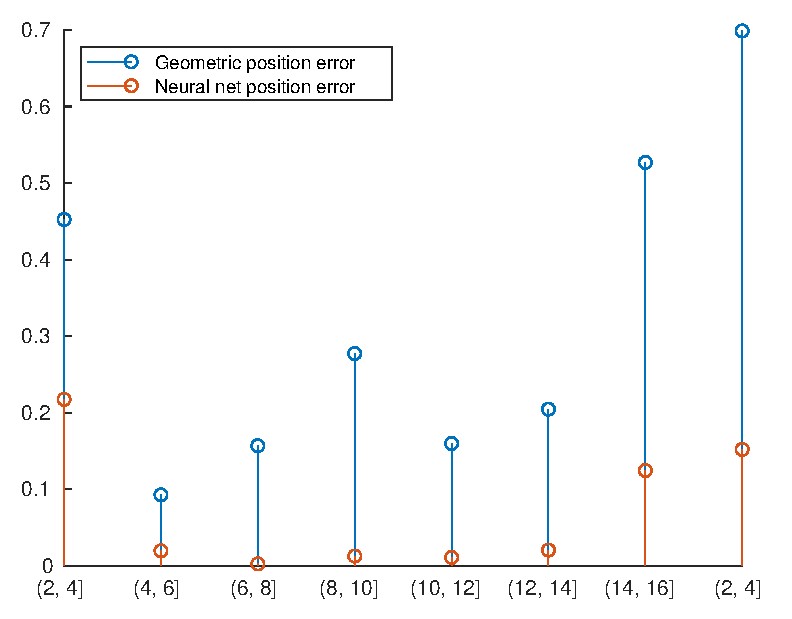
\includegraphics[width=0.5\linewidth]{0_Images/3_Theory/camDetection/psiErrorCamera.eps}
    %\captionof{figure}{The error and variance along the r-direction of the camera detection algorithm, using just geometric considerations on %the size of the .}
    \caption[Binned angle error from the camera detection algorithm.]
    {Binned angle error from the camera detection algorithm compared to ground truth. One is using just geometric calculations on the bounding box coming out of the neural net, while the other is a neural net that inputs the bounding box and the geometrically calculated position to give a better position estimate.}
    \label{Fig:CameraPsiError}
\end{figure}

\begin{figure}
    \centering
    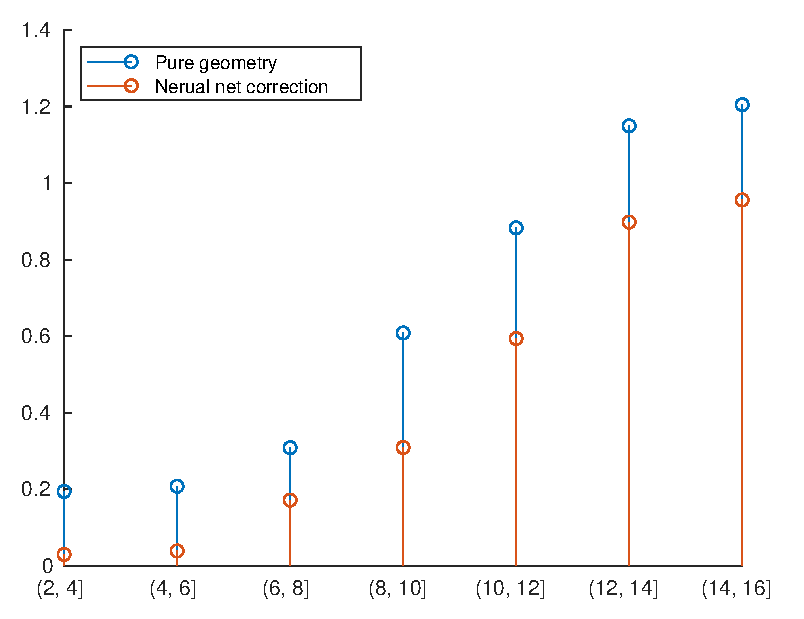
\includegraphics[width=0.5\linewidth]{0_Images/3_Theory/camDetection/rVarCamera.eps}
    %\captionof{figure}{The error and variance along the r-direction of the camera detection algorithm, using just geometric considerations on %the size of the .}
    \caption[Binned distance variance from the camera detection algorithm.]
    {Binned distance variance from the camera detection algorithm compared to ground truth. One is using just geometric calculations on the bounding box coming out of the neural net, while the other is a neural net that inputs the bounding box and the geometrically calculated position to give a better position estimate.}
    \label{Fig:CameraRVariance}
\end{figure}

\begin{figure}
    \centering
    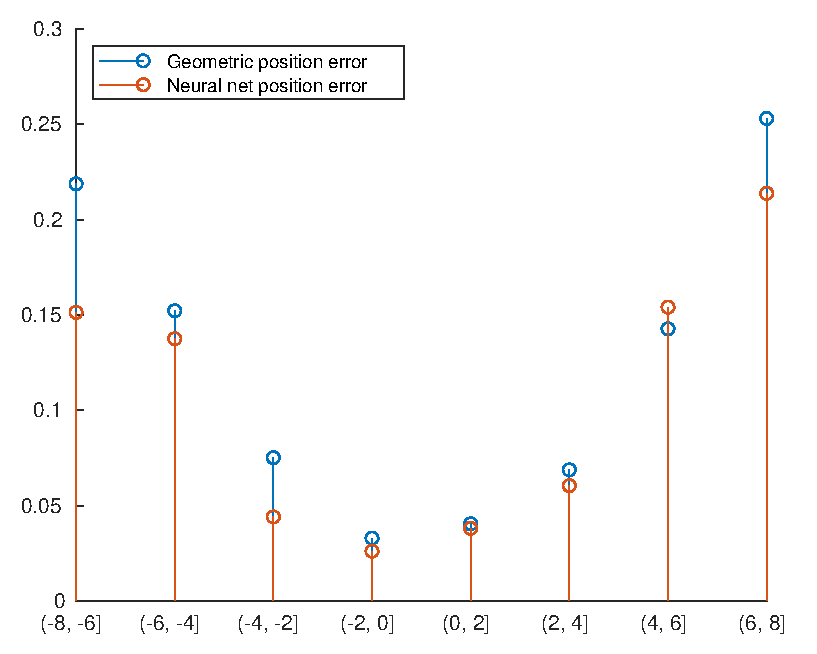
\includegraphics[width=0.5\linewidth]{0_Images/3_Theory/camDetection/psiVarCamera.eps}
    %\captionof{figure}{The error and variance along the r-direction of the camera detection algorithm, using just geometric considerations on %the size of the .}
    \caption[Binned angle variance from the camera detection algorithm.]
    {Binned angle variance from the camera detection algorithm compared to ground truth. One is using just geometric calculations on the bounding box coming out of the neural net, while the other is a neural net that inputs the bounding box and the geometrically calculated position to give a better position estimate.}
    \label{Fig:CameraPsiVariance}
\end{figure}

\begin{figure}
    \centering
    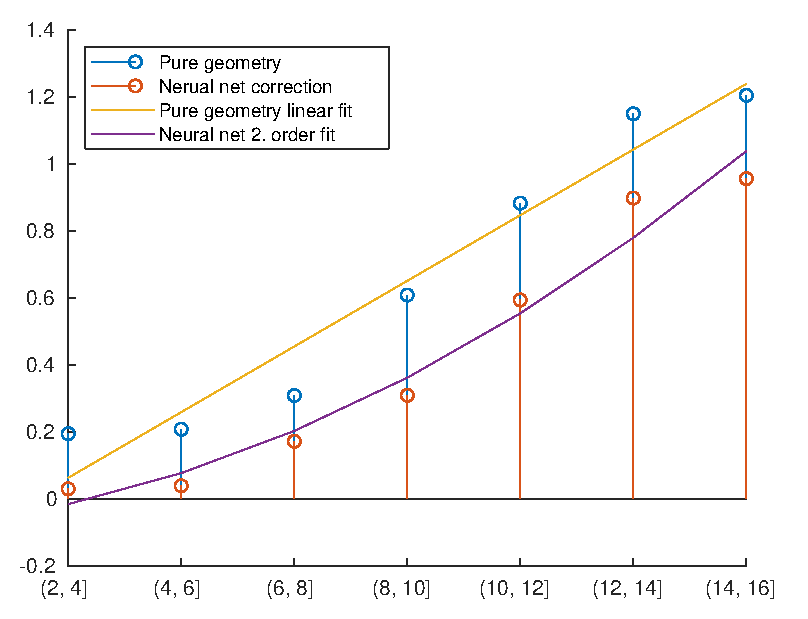
\includegraphics[width=0.5\linewidth]{0_Images/3_Theory/camDetection/CameraRVarianceFit.eps}
    %\captionof{figure}{The error and variance along the r-direction of the camera detection algorithm, using just geometric considerations on %the size of the .}
    \caption[Fitted functions over the r-variance of the camera detection algorithm.]
    {Fitted functions over the r-variance of the camera detection algorithm. The variance of the purely geometrically calculated distance is fitted linearly, while the neural net solution gets a second order polynomial.}
    \label{Fig:CameraRVarianceFit}
\end{figure}

\begin{figure}
    \centering
    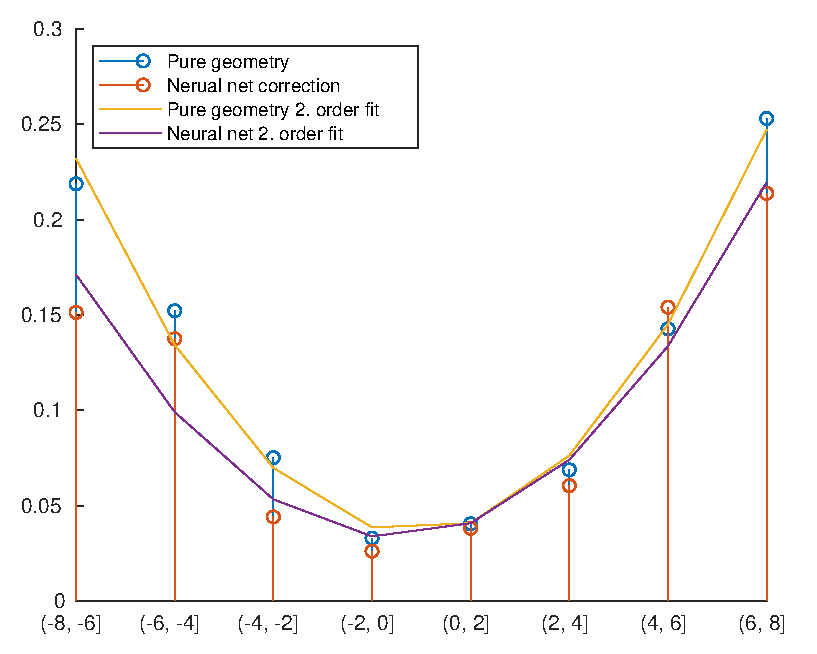
\includegraphics[width=0.5\linewidth]{0_Images/3_Theory/camDetection/CameraPsiVarianceFit.eps}
    %\captionof{figure}{The error and variance along the r-direction of the camera detection algorithm, using just geometric considerations on %the size of the .}
    \caption[Fitted functions over the $\psi$-variance of the camera detection algorithm.]
    {Fitted functions over the $\psi$-variance of the camera detection algorithm. Both the purely geometrically calculated value and the neural net solution got a second order fit.}
    \label{Fig:CameraPsiVarianceFit}
\end{figure}

\fi
\subsection{Comparison with the existing map}

Each detected cone is then transformed into the map frame, using the latest estimate of the cars position coming from the state estimation, as well as the correction on the state estimation that SLAM gives us. Since the last time a detection arrived, the state estimation covariance has been accumulated and is now added to all the landmarks in the map. 

This accumulation is simply summing of the diagonal covariance matrices of each odometry message, i.e. the covariance in the change of $x$, $y$ and $\psi$. This information arrives as covariances in the body frame, and even though this body frame will rotate and translate with respect to the map frame, it's assumed to never be a very long time between each set of detections arriving. Therefore it's assumed that the step from the last detection can be approximated as a single translation followed by a single rotation. This assumption is used to simplify the process of summing the covariances. 

Instead of integrating the covariance along the trajectory of the car, the covariance in $x$ and $y$ of the accumulated odometry is simply summed and rotated into the global frame before getting added to the covariance of each landmark in the map. This is of course a simplification, but it avoids having to iterate through the map each time a new odometry message arrives, which is at $\SI{400}{Hz}$, thus leading to a lot of unecessary computation. The team believes this error will be dominated by errors in the covariance estimates, so computation time was chosen over accuracy. 

The yaw covariance is accumulated by summing as well, but increases the covariance of each landmark in a different way. The covariance in yaw of the accumulated step will lead to an increased covariance of each landmark that is approximately aligned with the $\psi$-direction in the detection frame that sits on top of each landmark. The magnitude of this covariance is the accumulated covariance, $\sigma_{\psi}^2$ times the distance, $r$, between the landmark and the car. This leads to a covariance matrix in the detection frame, which is then rotated into the body frame and added to the covariance of the landmark

\begin{equation}
    \Sigma^{new} = \Sigma^{old} + R(\alpha)diag\{0,\sigma^2_{\psi}r\}
\end{equation}

Here $\Sigma^{old}$ is the old covariance of the landmark, $\Sigma^{new}$ is the new and $R(\alpha)$ is the rotation matrix aligning the detection frame with the body frame, defined in equation \ref{DetectToBodyRot}. 

The closest landmark in the map to each cone is then found, and a compatibility test is done for each detected cone, using the covariance of the detected cone and the covariance of the closest landmark. All positive associations are then sent to SLAM as new measurements to existing landmarks. This information also includes the pose the car was in when it saw the landmarks. 

Since the track follows some strict rules regarding spacing between landmarks, there will never be  cones too close together. Therefore each landmark has a safety zone around it of about $\SI{1}{meter}$. If a detection is within the safety radius of an already existing landmark, but doesn't pass the compatibility test with it, it gets discarded. This rule might mean discarding the few cones where this is not true, but it also makes the system overall more robust to outliers, so the team believes the trade off is worth it.  All the remaining detections are kept for comparison with the set of hypotheses. 

\subsection{Comparison with the set of hypotheses}

In the next step, the remaining detections are compared with the list of hyptheses. This is done the same way as for comparing with the map, by increasing the spatial covariance of all hypotheses, and association through a simple compatility test, where the Mahalanobis distance must be below a threshold. One major difference is however that if two detections from the same detection algorithm at the same time step can be associated to the same hypotheses, then both the measurements and the hypotheses are discarded as outliers. This simplification means no care must be taken with overlapping hypotheseses, like what is done in the JPDA. 

\subsubsection{Positive associations}

A positive association with a hypothesis means that the confidence of this hypothesis is increased, and the measurement is added to the list of measurements of this hypothesis. How much the confidence is increased was initially going to be a function of distance from the car, but the ratio between the number of false and true positives have so far not turned out to be dependent on distance or angle in any meaningfull way. For now the initial confidence is therefore just a function of which detection system the measurement came from. This is because there are fewer false positives from the camera algorithm than from the two LiDAR systems. 

A positive association also means that the position in the map frame of the hypothesis is updated by a Kalman update step. This is done by first finding the distance between the measured position $z_{k-1}$ and the estimated one, $\hat{x}_{k|k-1}$. Call this distance $\Tilde{x}_k$. To find the optimal weighting between the new measurement and the previous estimate, the so called Kalman gain, $K_k$, is created

\begin{equation}
    K_k = P_{k|k-1}S^{-1}_k
\end{equation}

where 

\begin{equation}
    S_k = R_k + P_{k|k-1}
\end{equation}

is the measurement noise, $R_k$, plus the propagated noise from the previous step, and $P_{k|k-1}$ is the covariance of the landmark. This gain is then used to give a high weight to the measurement when the measurement noise is low and system noise is high, and vice versa. The new estimated position of the landmark is then

\begin{equation}
    \hat{x}_{k|k} = \hat{x}_{k|k-1} + K_k\Tilde{y}_k
\end{equation}

The keen reader might notice that there is no $H_k$ in the above equation. This is because our measurement function is the identity. 

The new covariance, $P_{k|k}$, of the landmark is then found by  

\begin{equation}
    P_{k|k} = (I-K)(P_{k|k-1} + Q)
\end{equation}

This makes the covariance get smaller if the measurement and previous estimate are close together, and increase if they are far apart. In reality the covariance will always get smaller when a measurement is associated to a hypothesis, because of the compatibility test. 

\subsubsection{Lack of association}

If a hypothesis isn't associated to when a new set of detections arrive, its confidence is decreased. How much it's decremented by is a function of which detection system this set of detections came from, and whether or not this hypothesis is in the field of view of the detection system. If it is then the confidence is decremented by a number that is a function of distance. 

This last part has not been implemented yet, just like the initial confidence function, because we yet have no proper estimates of ratio between false positives and true positives as a function of distance. 

\subsubsection{Belief correction}

When a hypothesis' confidence climbs above a threshold it is accepted as an inlier and all the measurements of it are sent to SLAM as measurements of a new landmark. Similarily when the confidence goes below a threshold it is discarded. A hypothesis is also discarded when it's spatial gets too big. This is because we don't want ambiguity when associating measurements to the hypotheses. 

The remaining measurements are then initialized as a new hypothesis. It is given an initial confidence that is a function of detection method and distance from the car. This is because when we plot the ratio between true positive and false positives, this ratio goes down as the distance increases. Thus the confidence is initialized at a lower value when the cone is further away. 

